\documentclass[10pt,twocolumn,letterpaper]{article}

\usepackage{times}
\usepackage{epsfig}
\usepackage{graphicx}
\usepackage{float}
\usepackage{amsmath}
\usepackage{amssymb}
\usepackage{enumitem}
\usepackage{url}
\usepackage{cite}
\usepackage{multirow}

\usepackage[pagebackref=true,breaklinks=true,colorlinks,bookmarks=false]{hyperref}

\setlength\abovedisplayskip{1pt}
\setlength\belowdisplayskip{1pt}
\setlength\abovedisplayshortskip{1pt}
\setlength\belowdisplayshortskip{1pt}

\begin{document}

\title{Where Are They Really Looking?}

\author{
Ambika Verma\ \ \ Brady Zhou\\ \\
{\fontsize{11}{13}\selectfont University of Texas at Austin}\\
{\fontsize{10}{11}\selectfont \texttt{\{ambika,brady.zhou\}@utexas.edu}}
}

\maketitle

\begin{abstract}
    In this paper, we present a framework to predict where actors in an image are looking by utilizing joint attention and/or interaction characteristics. This approach is specifically useful in case of more than one person/actor being present in a scene. We use a combination of CNN \cite{nips15_recasens} and MRF \cite{fathi2012social} models to accomplish this task. The approach is motivated from recent state of the art work in Gaze Following (CNN) and Social Attention (MRF) domains.
\end{abstract}

\section{Introduction}

In our day to day life we tend to interact with people and/or objects in a fairly predictable manner specifically in terms of social attention and/or interaction such as we tend to notice things that a group of people might be attending to. Additionally our gaze (direction we look in) is a strong indication of what we might do next. Thus, it is imperative for a computer or robot trying to predict the type of actions or interactions occurring in an image or video, to follow gaze of actors in a scene effectively. As a result, gaze following can be used for different high level tasks such as predicting visual saliency, activity recognition, active perception and behavioural analysis.

As noted earlier we solely concentrate on gaze following task for multiple actors in an image or video, with the idea in mind that joint gaze prediction can benefit the task of gaze following since humans interact in a predictive manner. This leads to some of the assumptions made in this paper (which are derived from social attention domain) \cite{fathi2012social}, namely head orientation is a robust indicator of gaze direction and if another actor in the scene is looking at a particular location it is more likely for another person (with head orientation in the same direction) to be looking at it as well.

\subsection{Related Work}

As noted by \cite{nips15_recasens} there are only a few works which build upon the task of gaze following. There are three different scenarios where this task has been studied - Free-viewing Saliency, Social Attention/Interaction and true Gaze Following, we review each of tasks briefly in this section.

Identifying types of social attention and interactions occurring in a scene inherently limits itself to scenes with multiple people only \cite{fathi2012social} \cite{marin2014detecting} \cite{soo2015social}, \cite{soo2013predicting}, though, it boasts of intuitive methods to perform joint gaze prediction. \cite{fathi2012social} develops MRF and CRF methods for their task of predicting type of interaction taking place in a scene, which can be applied to long first-person videos to filter out useful clips or subsets (similar to video summarization). This work utilizes an MRF model to predict where people are looking in a scene to later classify the type of interaction taking place using CRF. Thus, gaze following is utilized in such techniques in an implicit manner. The model developed utilizes joint predictions effectively, though is heavily biased to look at other faces in the scene. This bias is acceptable for identifying the type of interaction amongst people but does not generalize well for the gaze following task, wherein actors can be looking at another actor or an object.

 On the other hand works in free-viewing saliency and gaze following tasks do include scenes with both multiple people and only one person. \cite{fathi2012social} is a CNN based model which is specifically tasked for gaze following utilizing head position and orientation along with saliency to accomplish the task.

 This method has several advantages, such as it is robust in case of single actor being present in a scene, does not suffer from any evident bias of looking at people only (such as in \cite{fathi2012social}) and the network architecture does not require extensive hand-crafted functions (such as those required in probabilistic models such as MRF or CRF). Even though, these merits are far reaching the model uses a naive approach in cases where multiple actors are present in the scene, it resorts to providing predictions for each actor individually.

 Another relevant work which utilizes gaze following is \cite{parks2015augmented} in which an actor’s gaze is used as an additional feature to generate more accurate free-viewing saliency maps. It has been noted in numerous works \cite{parks2015augmented},\cite{marin2014detecting},\cite{flom2007gaze}, \cite{emery2000eyes}, \cite{newman2000real} that the gaze of an actor in a scene influences where passive observers look during free-viewing. In this work the authors use head pose \cite{newman2000real} along with low level saliency \cite{garcia2012saliency} to predict more accurately the semantically salient regions in a scene. This work does utilize joint predictions in case of multiple actors in the scene and it is worthy to note that considerable performance improvement is achieved over state of the art saliency methods \cite{garcia2012saliency}. Even though this method can be extended to gaze following task, it has not been evaluated on the same.

 Works such as \cite{fathi2012social} and \cite{parks2015augmented} utilize gaze following and joint predictions to achieve a secondary task. Thus, our approach is to combine the works of \cite{fathi2012social} and \cite{nips15_recasens} in a constructive manner to add joint prediction capability to the model developed in \cite{fathi2012social} with the goal of achieving higher performance for cases with multiple actors in the scene.

\section{Technical Approach}

As in \cite{nips15_recasens} we also assume that the head positions are provided and as demonstrated in \cite{parks2015augmented} a head detector with pose estimation can be effectively used with a few modifications.

We plan to use the CNN network from \cite{nips15_recasens} with post-processing added through an MRF model which is designed on the lines of model used in \cite{fathi2012social} to account for joint gaze predictions. The overall architecture of our approach is illustrated in Fig 1.

\begin{figure*}[t]
  \begin{center}
    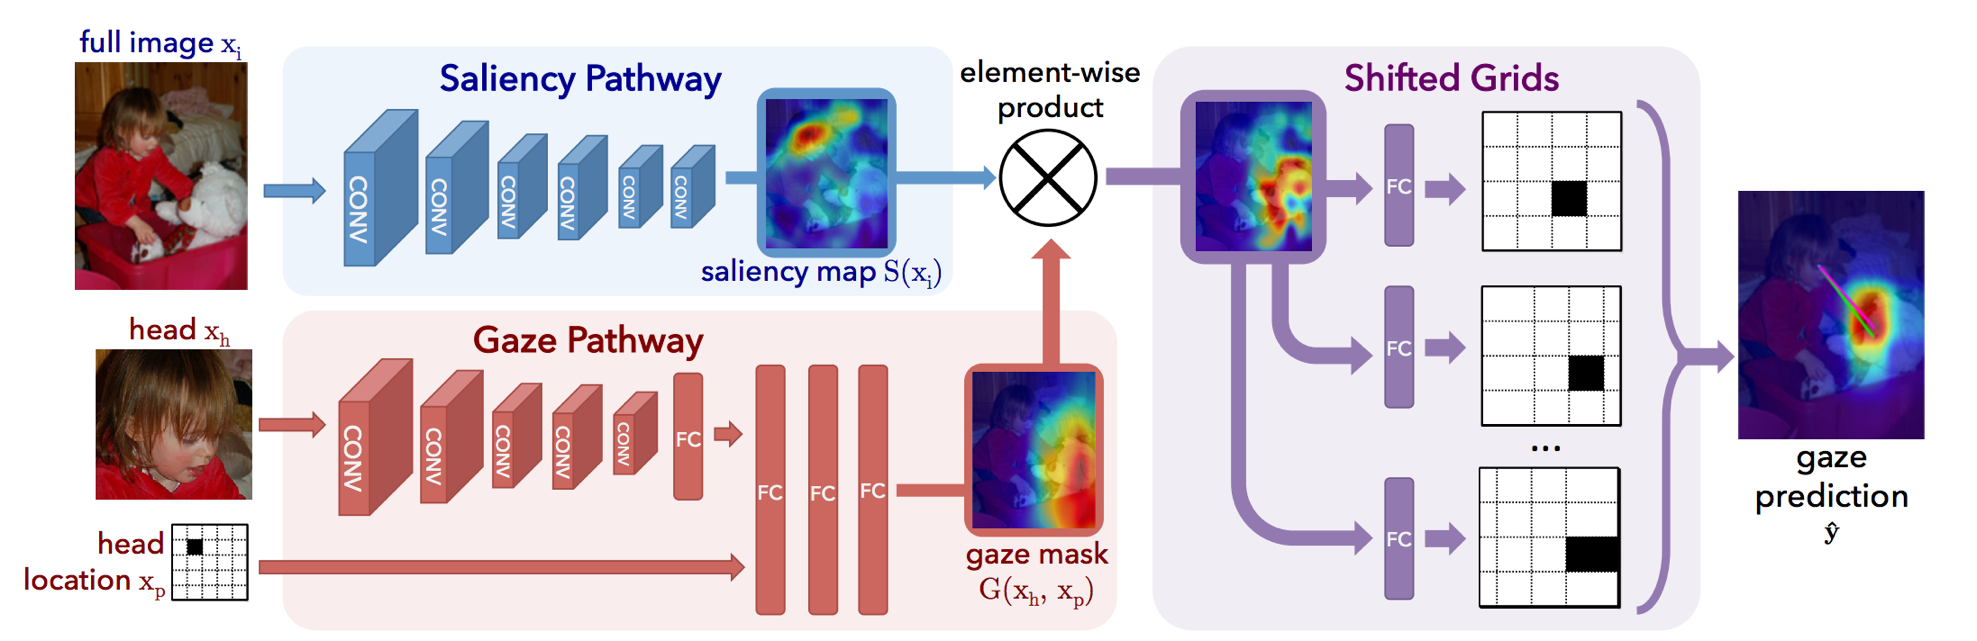
\includegraphics[width=0.95\linewidth]{images/cnn.png}
  \end{center}
  \vspace{-0.3cm}
   \caption{The network architecture from \cite{nips15_recasens}.}
  \vspace{-0.5cm}
\end{figure*}

A given image along with head position is provided as input to the CNN. We only use images where there are multiple actors in the scene. The CNN then iterates through the image for each actor and gives as an output a two-dimensional position $(g_x, g_y)$ normalized by the image dimensions to lie between 0 and 1. This prediction is then used as an initial seed for MRF model. In addition the MRF model is also supplied with head location and orientation vectors, where orientations is obtained using the head position along with predicted gaze location and is jittered to replicate errors one would observe using a head detector. The MRF model then optimizes the unary and pairwise potentials to jointly refine the CNN predictions based on the predictions obtained for other actors in the scene.

Following sections discuss the CNN and MRF models in detail.

\subsection{CNN Model}

The CNN model consists of two pathways, namely Gaze pathway and Saliency pathway. As noted in \cite{nips15_recasens}, the gaze pathway tends to learn predicting the direction of gaze based on the head orientation (this is the reason why we use the CNN prediction and head position to generate orientation vectors for the MRF model) and the saliency pathway tends to learn to find salient regions in the scene. The model is implemented in Caffe [] and the two pathways are equivalent to the first five layers of AlexNet \cite{krizhevsky2012imagenet}. The saliency pathway is initialized with weights from Places-CNN \cite{zhou2014learning} and gaze pathway is initialized with ImageNet-CNN \cite{russakovsky2015imagenet}.
The saliency and gaze masks obtained are then combined through an elementwise layer and final prediction is made through shifted grids. More details can be found in \cite{nips15_recasens}.

\subsection{MRF Model}

\textbf{Markov random fields} are a form of probabilistic graph models that have been heavily used throughout the computer vision field to solve classification problems \cite{wang2013markov}, \cite{quattoni2007hidden}. Markov random fields have proved to be effective in certain applications like image segmentation and parsing text (NLP).

\pagebreak

The goal of using an MRF is find a labeling $\{p_1 = l_1,\ p_2 = l_2,\ \dots,\ p_n = l_n\}$ such that the joint probability $P(p_1 = l_1,\ p_2 = l_2,\ \dots,\ p_n = l_n)$ is maximized.

\begin{figure}[H]
  \begin{center}
    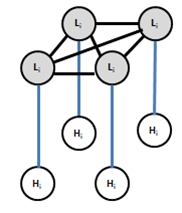
\includegraphics[width=0.3\linewidth]{images/mrf_model.png}
  \end{center}
  \vspace{-0.3cm}
   \caption{Markov random field depiction.}
  \vspace{-0.5cm}
\end{figure}


We use the graphical model from \cite{fathi2012social} to refine the gaze predictions from \cite{nips15_recasens}. The MRF model is used to utilize the relationship between the multiple actors in a scene. The motivation for this approach stems for example from scenes where multiple actors are looking at the same location. In case of individual predictions there is no way for benefitting from the information we have about the gaze of other actors in the scene, whereas joint prediction allows us to give higher weights to locations which lie in the direction of gaze of an actor and are also looked at by other actors in the scene.

The MRF model implementation uses the following unary and pairwise potentials. The unary potentials allows the model to predict the direction of the gaze based on head position and orientation vectors and on the other hand the pairwise potentials capture the interaction between actors in the scene. \\

\begin{equation}
  \phi_u = \phi_1 \cdot \phi_2 \cdot \phi_3
\end{equation}

The unary potential is a product over three different potential functions. Each of these potentials seeks to score the probability of a gaze (higher is better).

\begin{equation}
  \phi_1(l_i = l, d_i, f_i) = \frac{1}{\sigma \sqrt{2 \pi}} \exp{\big\{-\frac{\|d_i - (l - f_i)\|^2}{2 \sigma^2}\big\}}
\end{equation}

The first unary term is a guassian distribution of how well the predicted gaze aligns with the head orientation. This scores the labeling of a person $i$'s gaze to a location $l$. $l$ is a label, the cell of the predicted gaze. $d_i$ is a unit vector, the head orientation. $f_i$ is the position of the subject's face. $\sigma$ is a constant.

\begin{equation}
  \phi_2(l_i = l, f_i) = \frac{1}{1 + \exp{\{-c_t \cdot \|l - f_i\|\}}}
\end{equation}

The second unary term is a thresholding function that assigns the score to $0$ if the predicted gaze is too close to a person's face. This is used to prevent extremely short gazes (labeling a person's gaze to their own face). $c_t$ is a constant.

\begin{equation}
  \phi_3(l_i = l) = \begin{cases}
    c_p, & \text{if $l \in \{f_1,\ f_2,\dots,\ f_n\}$}.\\
    1, & \text{otherwise}.
  \end{cases}
\end{equation}

The third unary term is to bias subjects' gazes towards other faces in the scene. $c_p$ is a constant. \\

Next, MRFs, have a pairwise potential, a measure of how the assigned labels are related. In our model, the pairwise potentials model how one person's gaze affects another.

\begin{equation}
  \phi_P(l_i = l_1, l_j = l_2) = \begin{cases}
    c_e & \text{if $l_1 = l_2$}.\\
    1 - c_e & \text{otherwise}.
  \end{cases}
\end{equation}

The pairwise potential provides a bias towards looking at the same position in a scene. The constant $\frac{1}{2} \leq c_e \leq 1$ biases two gazes to the same cell.

The parameters $\sigma,\ c_t,\ c_p,\ c_e$ are learned through training images with more than one actor in the scene through cross validation.
Additionally, the image space which is the set of all possible gaze points is discretized into cells, we chose $50 \times 50$ empirically for performance reasons. With more cell sizes, we can have more fine grained predictions, but at $n = 50$ and greater, we see no significant difference in performance, and we can run the full pipeline in less than a second.

To perform energy minimization for the MRF, direct inference is intractable. The number of possible labelings for $n$ people using and a grid size of $25 \times 25$ is $ (25 \times 25)^n$. The complexity grows exponentially with the number of people with a high constant and a direct solver is not possible to use. We use a graph cut algorithm \cite{boykov2001fast} for approximate energy minimization that requires an initial labeling for each person. The method, alpha expansion, then iterate upon this initial labeling until convergence.

\section{Experiments}

\subsection{Dataset}

GazeFollow dataset \cite{nips15_recasens} is used as part of this work. The dataset contains 122,143 training images and 4,782 test images drawn from varied other datasets such as SUN \cite{xiao2010sun}, MS COCO \{lin2014microsoft, Actions 40 \cite{yao2011human}, PASCAL \cite{everingham2010pascal}, ImageNet challenge \cite{russakovsky2015imagenet}, and Places dataset \cite{zhou2014learning}.

Each image in training set is annotated with ground truth head position and ground truth gaze point.

Each image in test set is annotated with ground truth head position and 10 ground truth gaze points to account for human consistency. We use average of these 10 gaze points in all further experiments.

To assess performance on joint gaze prediction, we test our model on a subset of the GazeFollow dataset that contains multiple subjects.

The CNN model \cite{nips15_recasens} is trained on the GazeFollow dataset. 3500 images with multiple actors in the scene are used to train the MRF model and 1000 images are used for testing purpose.

\subsection{Evaluation Metrics}

We use two error metrics to quantify the performance of our method and to conduct comparative studies.

\textbf{$L_2$ distance} - The images are normalized to 1x1 and the distance between ground truth and predicted gaze point is taken. For a single image with multiple people, we report the average of the errors, that is -

\begin{equation}
\frac{1}{n} \sum_{i=1}^n \sqrt{(p_x^{(i)} - g_x^{(i)})^2 + (p_y^{(i)} - g_y^{(i)})^2}
\end{equation}

\textbf{Angular error} - The predicted gaze point is connected with the eye position to create a unit vector $v$, and the ground truth gaze point is connected with the eye position to create a unit vector $u$. The angular error is defined as $u^T v$, and converted to degrees.

\subsection{Baselines}

We evaluate the performance of the following models on the GazeFollow \cite{nips15_recasens} dataset. The goal of these experiments is to infer the learning carried out by the MRF model. This is achieved by varying the input applied to the MRF.

\begin{enumerate}[wide, labelwidth=!, labelindent=0pt, itemsep=0em]
  \item \textbf{Random} Random labels are assigned for each subject gaze point.
  \item \textbf{MRF-Chance} The input to the MRF model is set to random instead of using the CNN predictions. This allows us to gauge how useful the CNN predictions are.
  \item \textbf{MRF-Unary} The initial labels are obtained from optimizing the unary potentials. This is our implementation of \cite{fathi2012social}.
  \item \textbf{CNN} Equivalent to results obtained in \cite{nips15_recasens}.
  \item \textbf{Ours} We use the predictions from \cite{nips15_recasens} and use these in the MRF model from \cite{fathi2012social}.
  \item \textbf{Ours-Oracle} Our full model utilizing ground truth head position and orientations to quantify the model’s capability when provided with pristine inputs.
\end{enumerate}

\subsection{Quantitative Results}

\begin{figure}[H]
  \begin{center}
    \begin{tabular}{|l|r|r|}
      \hline
      Method & L2 Distance & Angular Error \\
      \hline
      Random & 0.452 & 67.12 \\
      MRF-Chance & 0.310 & 32.62 \\
      MRF-Unary & 0.278 & 28.43 \\
      CNN & 0.199 & 26.50 \\
      Ours & 0.266 & 26.82 \\
      Ours-Oracle & 0.210 & 15.58 \\
      \hline
    \end{tabular}
  \end{center}
  \vspace{-0.3cm}
   \caption{Quantitative comparisons between the gaze prediction models.}
  \vspace{-0.5cm}
\end{figure}

\vspace{3ex}
As expected random chance of assigning any point in the image space as the gaze point leads to high L2 and angular errors of 0.452 and 67.12 degrees respectively.  The CNN model achieves a performance of 0.1991 L2 distance and 26.5 degrees angular error. This is computed by iterating through each actor in a scene for the test images.

To test the MRF model we provide it with different inputs in terms of the initial labels as well as test its sensitivity to the head position and orientation information.  Comparing the results of MRF Chance (which has random initializations) and MRF Unary (initial labels computed using unary potentials)  with our model (CNN predictions as initial labels) strongly indicates the performance improvement by including the CNN predictions as initial labels and is illustrated in Fig. This also points in the direction that the MRF alone is not capable of capturing enough information from the head position and orientation only. The features learnt by CNN in terms of saliency and gaze maps capture orthogonal scene information which results in more robust predictions. Therefore, an MRF proves to be an ideal post-processing solution to account for joint gaze following predictions.

Furthermore, we compare the effect of head position and orientation accuracy on the overall performance of our full model. In one case we provide ground truth head position and orientation (computed using ground truth head position and gaze point) to our model and in another we add some gaussian random noise to the head position and orientation (computed using jittered head position and CNN prediction). For the oracle system we observe 0.21 L2 error and 15 degrees angular error compared to 0.27 and 26.8 degrees with noisy inputs. The accuracy of predictions is clearly sensitive to the accuracy of the head position and orientation values. Additionally the angular error is affected to a higher extent than L2 error, illustrating the close relationship between head orientation and gaze direction. This result is in accordance to the work in \cite{nips15_recasens} wherein the authors compare the predictions when no head information is used versus no image information.

\begin{figure}[H]
  \begin{center}
    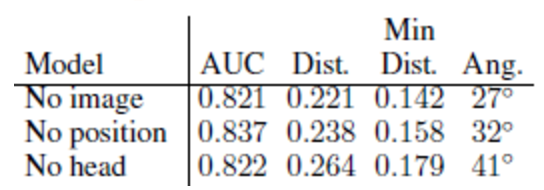
\includegraphics[width=0.75\linewidth]{images/head_table.png}
  \end{center}
  \vspace{-0.3cm}
   \caption{CNN performance given different head information \cite{nips15_recasens}.}
  \vspace{-0.5cm}
\end{figure}

\vspace{3ex}
Looking at the above mentioned performance results, specifically CNN versus our full model, the overall performance is similar for both cases. Thus, to investigate this further and to ascertain if the MRF model has learnt some intelligent features we divide the set of test images into two subsets, namely images with good CNN predictions and those with bad CNN predictions. A threshold on L2 and angular error is applied to populate these two sets. The corresponding performance results for these subsets are shown in Figure 5.

\begin{figure}[H]
  \begin{center}
    \begin{tabular}{|l|r|r|r|r|}
      \hline
      Method & L2 A & Ang. A & L2 B & Ang. B \\
      \hline
      Bad CNN & 0.38 & 41.29 & 0.23 & 21.28 \\
      Good CNN & 0.18 & 11.09 & 0.21 & 13.71 \\
      \hline
    \end{tabular}
  \end{center}
  \vspace{-0.3cm}
   \caption{Results on various thresholded subsets of the data. A corresponds to the CNN results and B corresponds to our method.}
  \vspace{-0.5cm}
\end{figure}

\vspace{3ex}
The performance results on these subsets lead to the following observations. For the set with bad CNN predictions the MRF is clearly able to refine the gaze point predictions based on joint distributions.  In the case of good CNN predictions the MRF model still tries to correct these even though the results from CNN model are fairly accurate with respect to the ground truth.

From the above observations we can conclude that the full model suffers when the CNN predictions are fairly accurate and therefore does not know when to stop correcting the inputs provided. This can also possibly point towards an overfitting scenario for the MRF model wherein it always implicitly assumes the input gaze point labels to be inaccurate.

\subsection{Qualitative Results}

Qualitative results are presented on the last page. We can see that the success cases consist of images where people are looking at other people, which validates that the unary potentials work well. The failure cases consist of images where there is a face closely aligned to the head orientation vector. In these cases, the third unary term that biases faces would pull the predicted gaze closer to the face.

\begin{table*}[ht]
  \centering
  \begin{tabular}{|c|c|}
    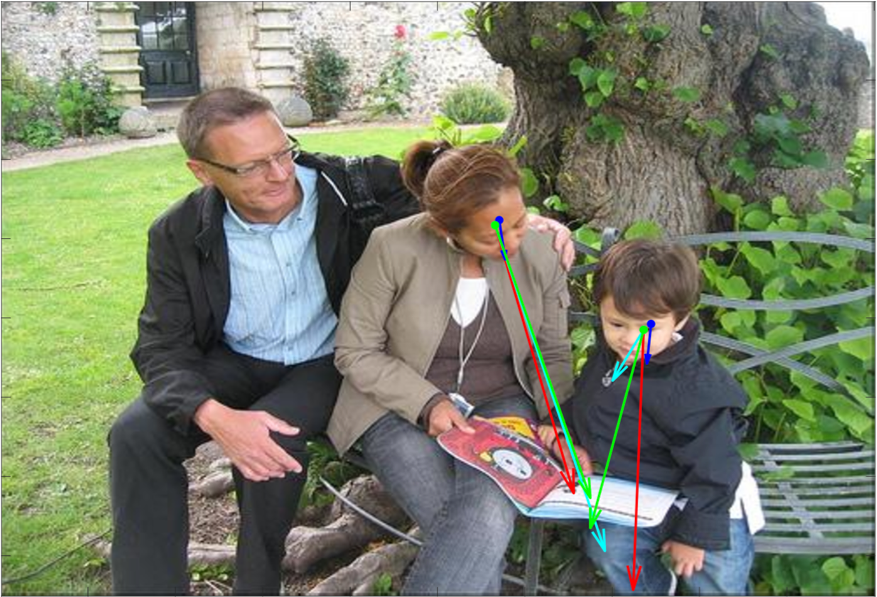
\includegraphics[width=55mm]{images/success1.png} & 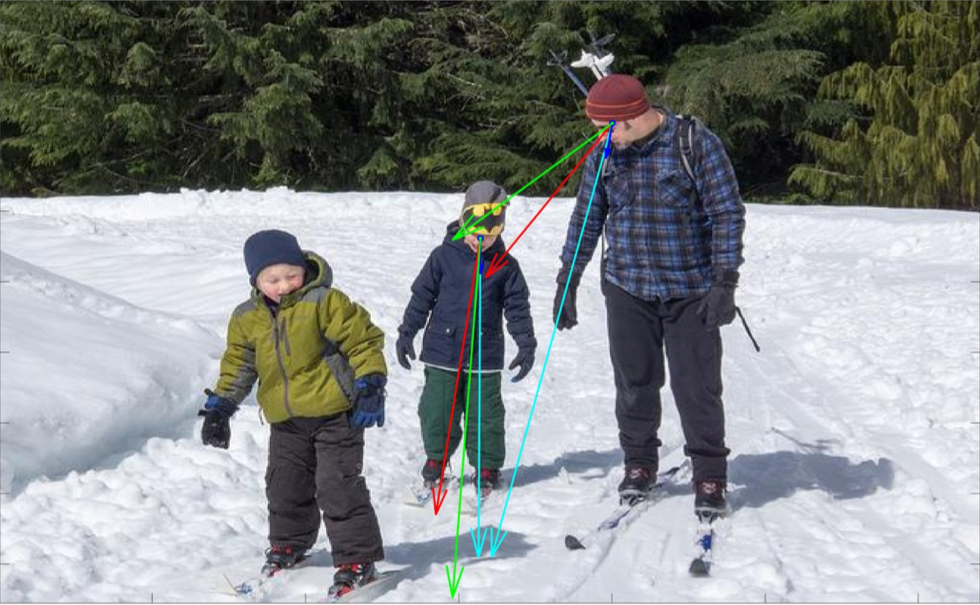
\includegraphics[width=55mm]{images/success2.png} \\
    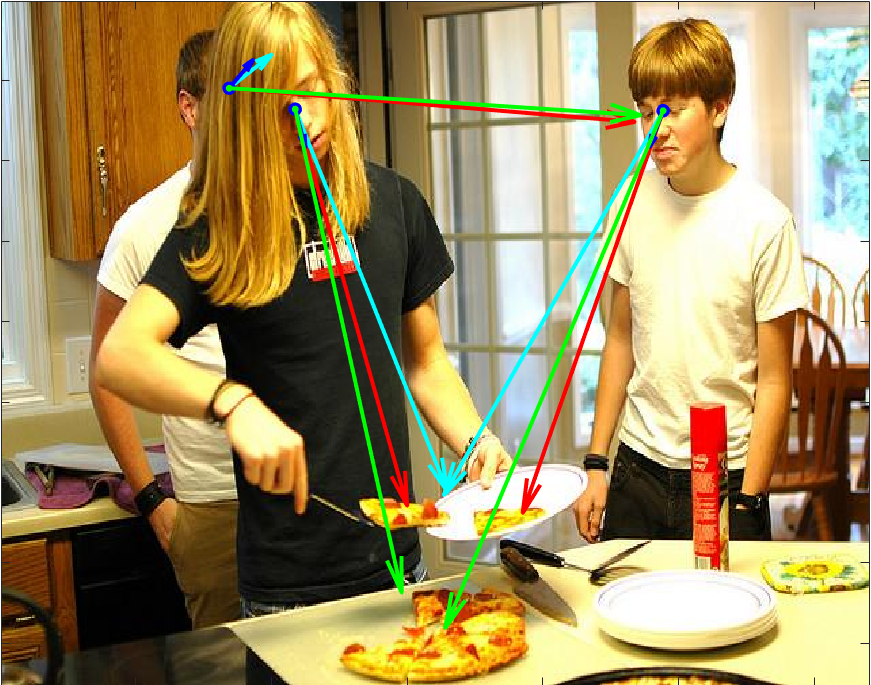
\includegraphics[width=55mm]{images/success3.png} & 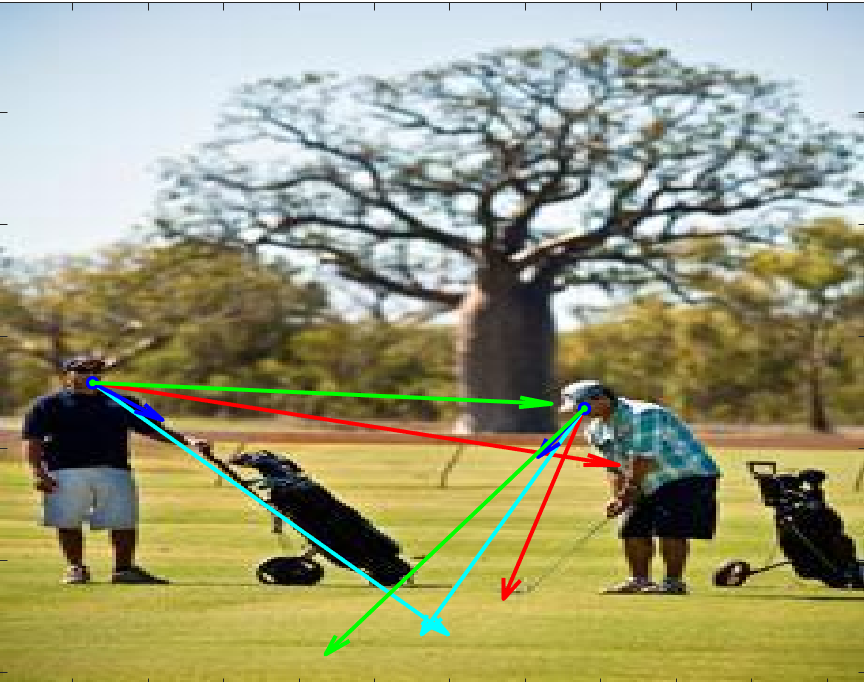
\includegraphics[width=55mm]{images/success4.png} \\
    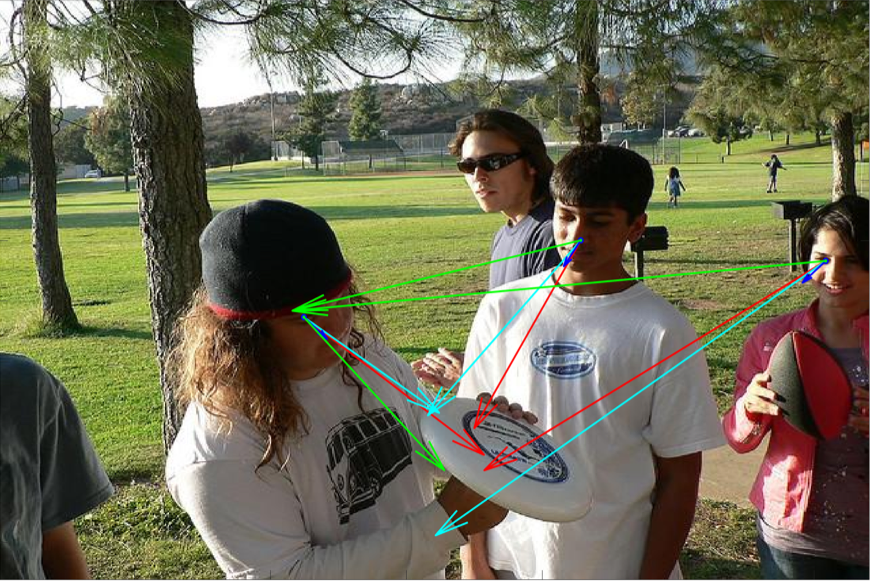
\includegraphics[width=55mm]{images/failure1.png} & 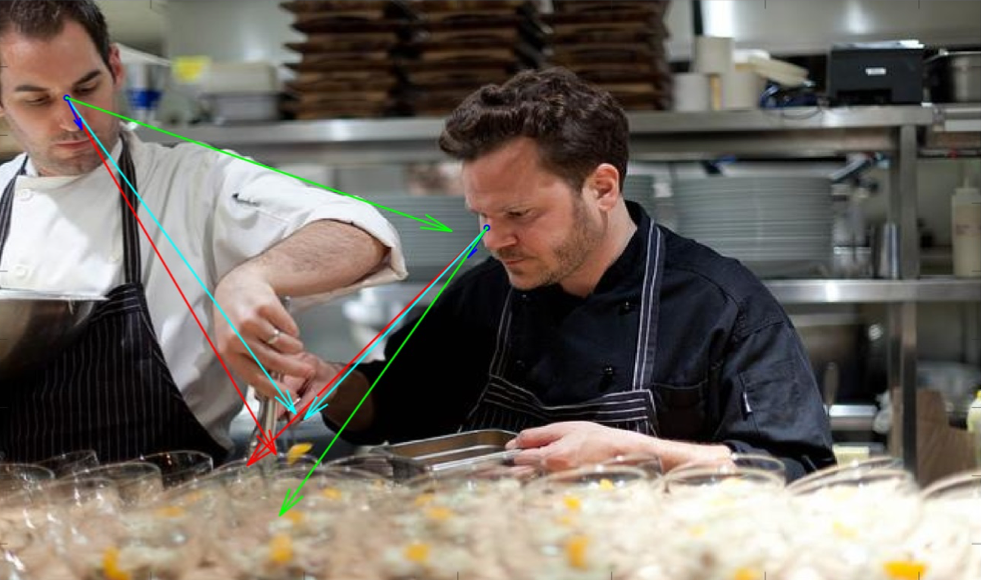
\includegraphics[width=55mm]{images/failure2.png} \\
    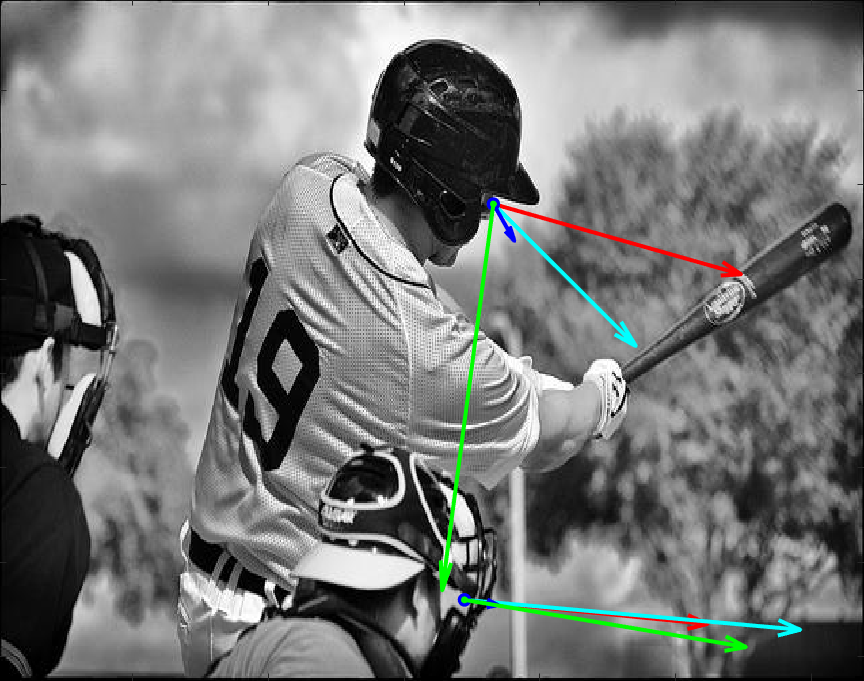
\includegraphics[width=55mm]{images/failure3.png} & 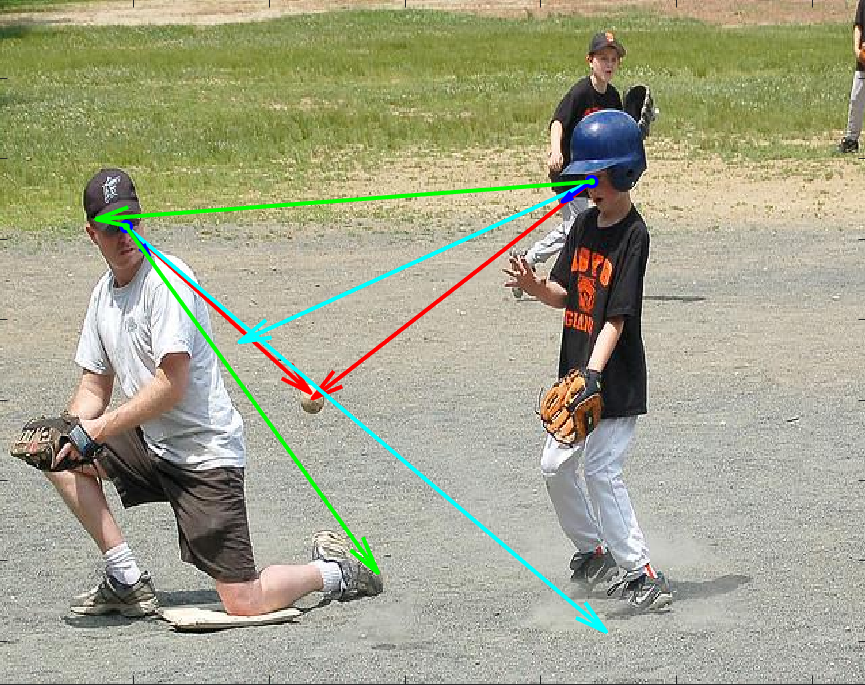
\includegraphics[width=55mm]{images/failure4.png} \\
  \end{tabular}

  \caption{Ground truth plotted in red. CNN predictions plotted in blue. Ours plotted in green. The top two rows show success cases of capturing mutual gazes. The bottom two rows show failure cases.}
\end{table*}

\section{Conclusion}

We explored an approach to combine and utilize two state of the art methods, GazeFollow model \cite{nips15_recasens} and Social Attention \cite{fathi2012social} for gaze following task specifically in the case of multiple actors in a scene. In the MRF model unary and pairwise potentials are formulated to account for head pose of an actor and relationship between actors respectively in a scene.

From the experiments conducted it is clear that the MRF model directly benefits from initial labels sourced from CNN predictions. Additionally, our model is more sensitive to the head position and orientation accuracy, similar to results obtained in \cite{nips15_recasens} (shown in Fig 4.)

\subsection{Further Extensions}

In performance analysis we noticed that most gazes are overshooting the ground truth gaze point, and we have pinpointed the cause to one of the unary potential terms. The potential function $phi_1$ seeks to align the gaze prediction point with the head orientation will always choose to pick a further point along a given gaze vector due to the discretization of the grid. Further points will be more aligned with the head orientation and therefore have a higher score. Future work would include exploring robust potential functions such as Gaussian distribution of gaze vector length.

An important direction to go in for further enhancing the method is to allow the model to dynamically decide between further refining the input CNN predictions and going back to the given input if further refinement is deleterious. Additionally, a holistic approach would be to integrate joint prediction mechanism with the CNN model from \cite{nips15_recasens}, which would result in a more robust and accurate network than combining two different techniques.

{\small
\bibliography{paper}
\bibliographystyle{IEEEtran}
}

\end{document}
